%---------------------------------------------------------------
%	PACKAGES AND OTHER DOCUMENT CONFIGURATIONS
%---------------------------------------------------------------

\documentclass[11pt,fleqn]{book} % Default font size and left-justified equations

\input{structure.tex} % Insert the commands.tex file which contains the majority of the structure behind the template

\hypersetup{pdftitle={Math Analysis Notes},pdfauthor={Noah Love}} 

%---------------------------------------------------------------

\begin{document}

%---------------------------------------------------------------
%	TITLE PAGE
%----------------------------------------------------------------

\begingroup
\thispagestyle{empty} % Suppress headers and footers on the title page
\begin{tikzpicture}[remember picture,overlay]
\node[inner sep=0pt] (background) at (current page.center) {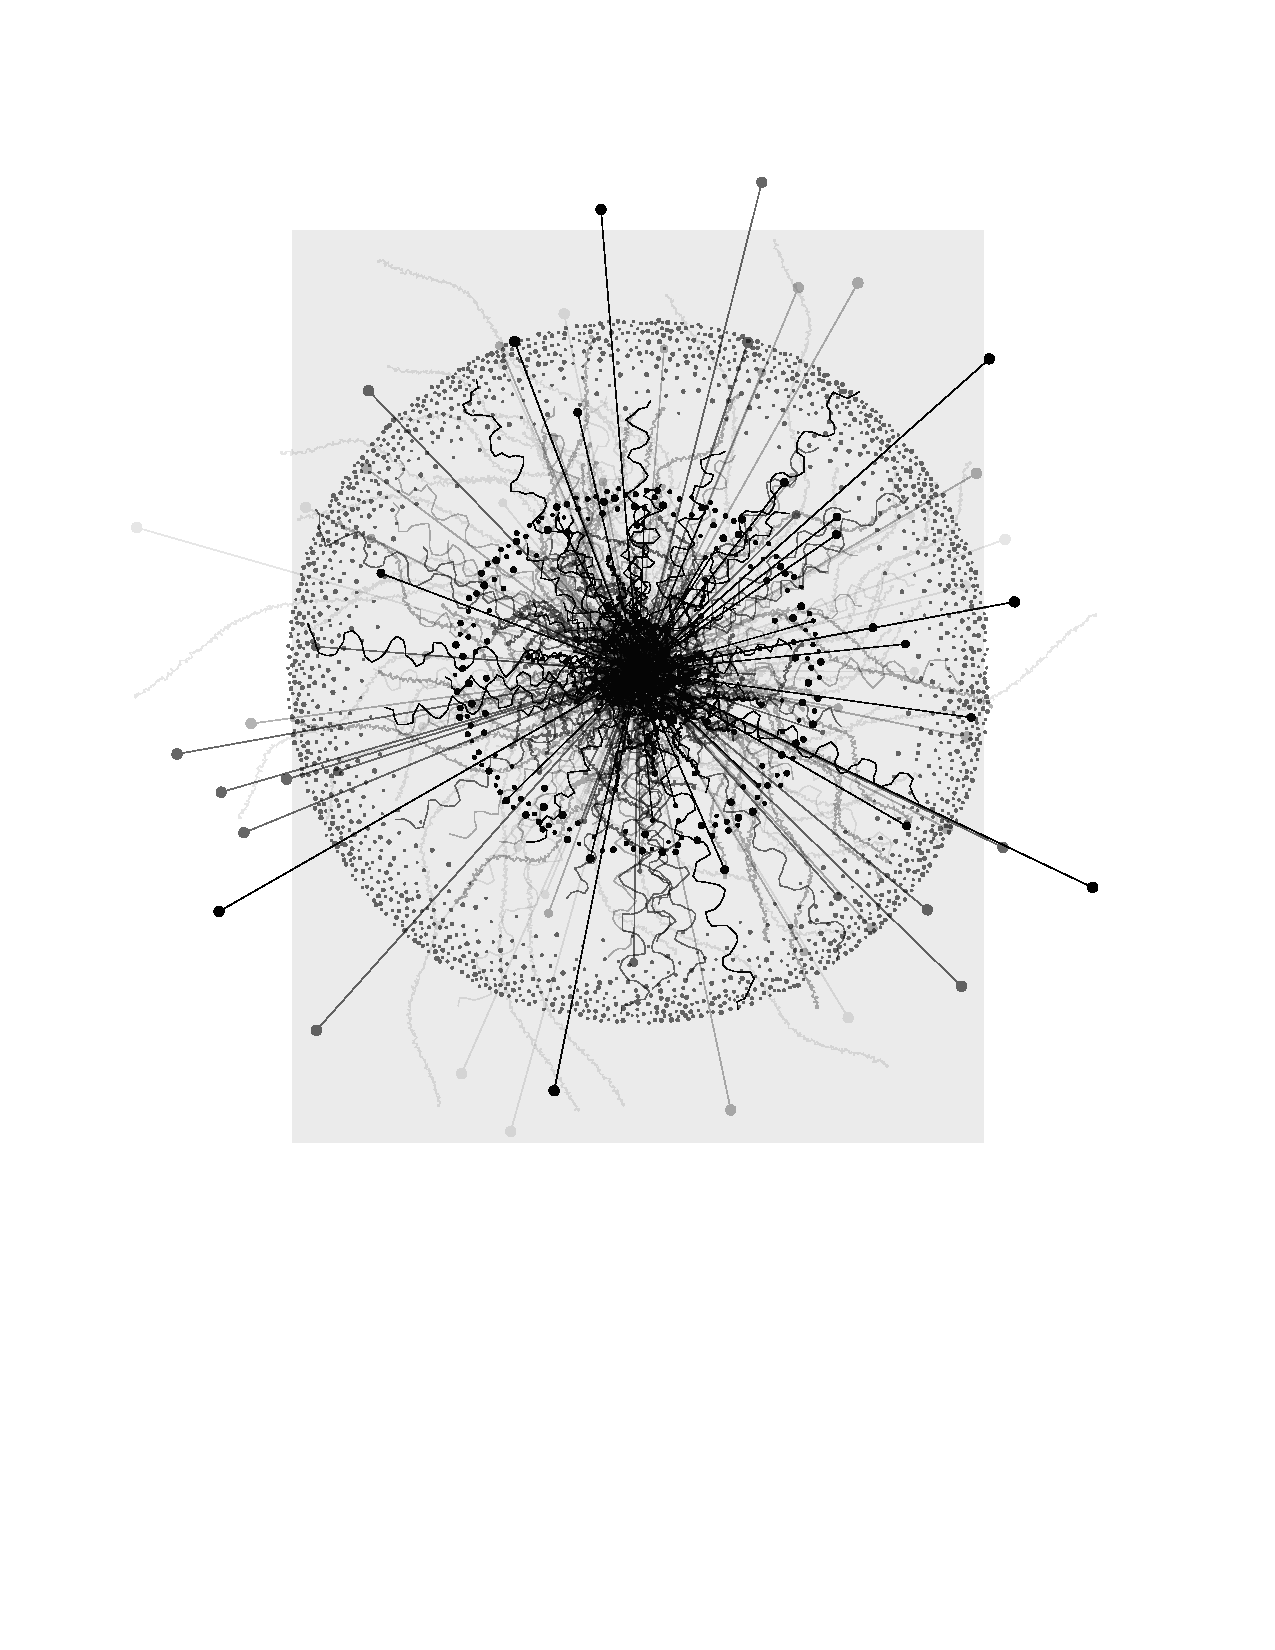
\includegraphics[width=\paperwidth]{background.pdf}};
\draw (current page.center) node [fill=white,fill opacity=0.6,text opacity=1,inner sep=1cm]{\Huge\centering\bfseries\sffamily\parbox[c][][t]{\paperwidth}{\centering TITLE\\[15pt] % Book title
{\Large Columbia University}\\[20pt] % Subtitle
{\huge Noah Love}}}; % Author name
\end{tikzpicture}
\vfill
\endgroup

%-------------------------------------------
%	COPYRIGHT PAGE
--------------------------------------------------

\newpage
~\vfill
\thispagestyle{empty}

\noindent Copyright \copyright\ YEAR Noah Love\\ % Copyright notice

\noindent \textsc{Class taught by PROFESSOR NAME}\\ % Publisher

\noindent \textsc{noah.love@columbia.edu}\\ % URL

\noindent Licensed under the Creative Commons Attribution-NonCommercial 3.0 Unported License (the ``License''). You may not use this file except in compliance with the License. You may obtain a copy of the License at \url{http://creativecommons.org/licenses/by-nc/3.0}. Unless required by applicable law or agreed to in writing, software distributed under the License is distributed on an \textsc{``as is'' basis, without warranties or conditions of any kind}, either express or implied. See the License for the specific language governing permissions and limitations under the License.\\ % License information, replace this with your own license (if any)

\noindent \textit{Columbia University YEARS} % Printing/edition date

\noindent \textit{Written in \LaTeX} % Printing/edition date

%-------------------------------------------------------------
%	TABLE OF CONTENTS
%---------------------------------------------------------------

%\usechapterimagefalse % If you don't want to include a chapter image, use this to toggle images off - it can be enabled later with \usechapterimagetrue

\chapterimage{The core} % Table of contents heading image

\pagestyle{empty} % Disable headers and footers for the following pages

\tableofcontents % Print the table of contents itself

\cleardoublepage % Forces the first chapter to start on an page so it's on the right side of the book

\pagestyle{fancy} % Enable headers and footers again

%-------------------------------------------------------------
%	PART
%------------------------------------------------------------



% \part{Midterm 1}

%--------------------------------------------------------------
%	CHAPTER 1
%--------------------------------------------------------------

\chapter{Math Review}

\section{Notation}
This is an important section so that you can understand all of the following information. Although typically written in English, mathematicians have their own language and that is a language of signs. 

The most important symbol to know is: 


$$\mathbb{Z}$$



% The ordering of these symbols is slightly odd.  This is because I had to put all the
% long pieces of text in the same column (the right) for it all to fit properly.
% Otherwise, it wouldn't be possible to fit four columns of symbols here.

\begin{tabular}{@{}l@{\hspace{1ex}}l@{\hspace{1em}}l@{\hspace{1ex}}l@{\hspace{1em}}l@{\hspace{1ex}} l@{\hspace{1em}}l@{\hspace{1ex}}l@{}}
$\leq$          &  \verb!\leq!  &
$\geq$          &  \verb!\geq!  &
$\neq$          &  \verb!\neq!  &
$\approx$       &  \verb!\approx!  \\
$\times$        &  \verb!\times!  &
$\div$          &  \verb!\div!  &
$\pm$           & \verb!\pm!  &
$\cdot$         &  \verb!\cdot!  \\
$^{\circ}$      & \verb!^{\circ}! &
$\circ$         &  \verb!\circ!  &
$\prime$        & \verb!\prime!  &
$\cdots$        &  \verb!\cdots!  \\
$\infty$        & \verb!\infty!  &
$\neg$          & \verb!\neg!  &
$\wedge$        & \verb!\wedge!  &
$\vee$          & \verb!\vee!  \\
$\supset$       & \verb!\supset!  &
$\forall$       & \verb!\forall!  &
$\in$           & \verb!\in!  &
$\rightarrow$   &  \verb!\rightarrow! \\
$\subset$       & \verb!\subset!  &
$\exists$       & \verb!\exists!  &
$\notin$        & \verb!\notin!  &
$\Rightarrow$   &  \verb!\Rightarrow! \\
$\cup$          & \verb!\cup!  &
$\cap$          & \verb!\cap!  &
$\mid$          & \verb!\mid!  &
$\Leftrightarrow$   &  \verb!\Leftrightarrow! \\
$\dot a$        & \verb!\dot a!  &
$\hat a$        & \verb!\hat a!  &
$\bar a$        & \verb!\bar a!  &
$\tilde a$      & \verb!\tilde a!  \\

$\alpha$        &  \verb!\alpha!  &
$\beta$         &  \verb!\beta!  &
$\gamma$        &  \verb!\gamma!  &
$\delta$        &  \verb!\delta!  \\
$\epsilon$      &  \verb!\epsilon!  &
$\zeta$         &  \verb!\zeta!  &
$\eta$          &  \verb!\eta!  &
$\varepsilon$   &  \verb!\varepsilon!  \\
$\theta$        &  \verb!\theta!  &
$\iota$         &  \verb!\iota!  &
$\kappa$        &  \verb!\kappa!  &
$\vartheta$     &  \verb!\vartheta!  \\
$\lambda$       &  \verb!\lambda!  &
$\mu$           &  \verb!\mu!  &
$\nu$           &  \verb!\nu!  &
$\xi$           &  \verb!\xi!  \\
$\pi$           &  \verb!\pi!  &
$\rho$          &  \verb!\rho!  &
$\sigma$        &  \verb!\sigma!  &
$\tau$          &  \verb!\tau!  \\
$\upsilon$      &  \verb!\upsilon!  &
$\phi$          &  \verb!\phi!  &
$\chi$          &  \verb!\chi!  &
$\psi$          &  \verb!\psi!  \\
$\omega$        &  \verb!\omega!  &
$\Gamma$        &  \verb!\Gamma!  &
$\Delta$        &  \verb!\Delta!  &
$\Theta$        &  \verb!\Theta!  \\
$\Lambda$       &  \verb!\Lambda!  &
$\Xi$           &  \verb!\Xi!  &
$\Pi$           &  \verb!\Pi!  &
$\Sigma$        &  \verb!\Sigma!  \\
$\Upsilon$      &  \verb!\Upsilon!  &
$\Phi$          &  \verb!\Phi!  &
$\Psi$          &  \verb!\Psi!  &
$\Omega$        &  \verb!\Omega!  
\end{tabular}
\footnotesize







%--------------------------------------------------------------
%	Linear Algebra Review
%--------------------------------------------------------------




\chapter{Review of Linear Algebra}

\section{Matrices}

\begin{definition}
	A $m \times n$ matrix is a rectuangular array with m rows and n columns:
	\begin{equation}
		\mathbf{A} = (a_{ij})_{m \times n} = \begin{pmatrix}
			a_{11} & a_{12} & \dots & a_{1n} \\
			a_{21} & a_{22} & \dots & a_{2n} \\
			\vdots & \vdots &  \ddots & \vdots \\
			a_{m1} & a_{m2} & \dots & a_{mn} 
		\end{pmatrix}
	\end{equation}
\end{definition}

Above we have $m \times n$ individual entries, each of which can be identified by $a_{ij}$ where i is the row and j is the column it is located in. 

THis is a test to see if it ever redoes it. Does this work?

\subsection{Matrix Operations}

Let's assume that we have two equal dimension matrices:
\begin{equation}
	\mathbf{A} = (a_{ij})_{m \times n }, \quad \mathbf{B} = (b_{ij})_{m \times n }
\end{equation}


\section{Partitioned Matrices}

\section{Inverses}

\section{Linear Independence}

\section{Rank of a matrix}

\section{Results from Linear Systems}

\section{Eigenvalues and Eigenvectors}

\begin{definition}
	An eignevector of $A_{n \times n}$ is a nonzero vector $x$ satisfying 
	\begin{equation}
		Ax = \lambda x
	\end{equation}
	for some $ \lambda \in \mathbb{C}$. The associated value $\lambda$ is called the eigenvalue. 
\end{definition}

\begin{example}
	\begin{equation}
		A = \begin{pmatrix}
			a_{11} & a_{12} \\
			1_{21} & a_{22}
		\end{pmatrix} \Rightarrow (A - \lambda I) x = 0
	\end{equation}
	For this to be true, $(A - \lambda I)$ must have a non-zero determinent. In the case above:
	\begin{equation*}
		\begin{pmatrix}
			a_{11} - \lambda & a_{12} \\
			a_{21} & a_{22} - \lambda			
		\end{pmatrix} =  \lambda^2 - (a_{11} + a_{22}) \lambda + (a_{11}a_{22} - a_{12}a_{21}) = 0
	\end{equation*} 
	Then for the roots, we have:
	\begin{align}
		\lambda_1 + \lambda_2 = a_{11} + a_{22} = \text{tr}(A) \\ 
		\lambda_1 \lambda_2 = a_{11} a_{22} - a_{12} a_{21} = \text{det} (A)
	\end{align}
\end{example}

\begin{example}
	\begin{equation*}
		\begin{pmatrix}
			1 & 2 \\
			3 & 0
		\end{pmatrix} \Rightarrow \lambda^2 - \lambda - 6 = 0  = (\lambda - 3)(\lambda + 2)
	\end{equation*}
	From this, we know the $\lambda$ values are 3  and -2. From here, we have the equations:
	\begin{align*}
		x_1 + 2x_2 = 2x_1 \\
		3x_1 + 0 = 3x_2
	\end{align*}
	From this: we see that $x_1$ = $x_2$ meaning there  is an infinite amount of eigenvectors. They can be written generally as:
	\begin{equation*}
		x = \begin{pmatrix}
			t \\
			t
		\end{pmatrix}
	\end{equation*}
	For the case where $\lambda = -2$
	we have the equations:
	\begin{align*}
		x_1 + 2x_2 = 2 x_1 \\
		3x_1 + 0 = -2x_2
	\end{align*}
	Then we  get a similar equation:
	\begin{equation*}
		x = \begin{pmatrix}
			-2/3 t \\
			t
		\end{pmatrix}
	\end{equation*}
	Again there is an infinite amount because you can multiple by a scalar. 
\end{example}


In general:
\begin{equation}
	Ax = \lambda x \iff (A - \lambda I) x = 0 \iff det(A - \lambda I) = 0
\end{equation}

\begin{definition}[characteristic polynomial]
	\begin{equation*}
		p(\lambda)  = det(A - \lambda I) = (-\lambda)^n + b_{n-1}(-\lambda)^{n-1} + \dots + b_1 (-\lambda) + b_0
	\end{equation*}
	The zeros of the characteristic polynomial are precisely the eigenvalues of $A$. 
\end{definition}


\section{Quadratic Forms}

\section{Quadratic Forms with Linear Constraints}



%------------------------------------------------------------
%	INDEX
%---------------------------------------------------------------



\cleardoublepage % Make sure the index starts on an odd (right side) page
\phantomsection
\setlength{\columnsep}{0.75cm} % Space between the 2 columns of the index
\addcontentsline{toc}{chapter}{\textcolor{ocre}{Index}} % Add an Index heading to the table of contents
\printindex % Output the index

%----------------------------------------------------------------

\end{document}
